\documentclass{sig-alternate}
\usepackage{algorithm,algorithmic}
\usepackage{times}
\usepackage{cite}
\usepackage{graphicx}
\usepackage{url}
\usepackage{subfigure}
\usepackage{amsthm}

\newcommand{\vectort}{\mathbf{t}}
\newcommand{\vectortstar}{\mathbf{t}^*}
\newcommand{\vectorx}{\mathbf{x}}
\newcommand{\vectory}{\mathbf{y}}
\newcommand{\matrixB}{\mathbf{B}}
\newcommand{\vectortau}{\boldsymbol{\tau}}
\newcommand{\vectorp}{\mathbf{p}}
\newcommand{\setR}{\mathbb{R}}

\renewcommand{\algorithmicrequire}{\textbf{Input:}}
\renewcommand{\algorithmicensure}{\textbf{Output:}}
\renewcommand{\algorithmiccomment}[1]{  /* #1 */}
\newcommand{\BEGIN}{\item[\textbf{Begin}]}
\newcommand{\END}{\item[\textbf{End}]}

\newtheorem{thm}{Theorem}

\newcommand{\db}[1]{\raisebox{1ex}[0pt]{#1}}
\renewcommand{\arraystretch}{1.5}

\title{Simulation-Based Circuit Modeling with Convex Tensor-Product B-Splines
}

\author{\\ \\ \\ \\
%First Author\\
%Institution\\
%First line of institution address\\ Second line of institution address\\ 
%FirstAuthor@institution.com\\
% For a paper whose authors are all at the same institution, 
% omit the following lines up until the closing ``}''.
% Additional authors and addresses can be added with ``\and'', 
% just like the second author.
\and
\\ \\ \\ \\
%Second Author\\
%Institution2\\
%First line of institution2 address\\ Second line of institution2 address\\ 
%SecondAuthor@institution2.com\\
}

\begin{document}
\maketitle

\begin{abstract}
Convex fitting is essential for simulation-based circuit modeling
when convex programming is involved in an optimization process for 
applications such as analog circuit sizing or gate sizing. 
Inspired by the works in
computer-aided geometric design, a tensor-product B-spline based
modeling method is proposed. 
The main advantage of using B-spline is that convexity can
be retained by simply enforcing its control polygon. It turns out
that the convex fitting problem itself can be formulated as a convex
programming, and hence can be solved efficiently and globally.
Circuit design examples are given to demonstrate the
practicability of the proposed method.
%% Modeling the performance and characteristic functions of circuits is
%% extensively applied in the field of design automation. 
%% To derive SPICE-level accurate functions in a straightforward style,
%% tensor-product B-spline approximation method is proposed.
%% In order to preserve the convexity of original circuit
%% characteristic, the shape preserving and variation diminishing
%% properties of B-spline are explored and semidefinite
%% programming is employed in the approximation, hence the coefficients
%% of B-splines form a convex polygon arc. Finally circuit design example
%% demonstrates the practicability of the proposed method.
% Luk: Why circuit characteristic has to be convex?
\end{abstract}

\section{Introduction}
This work was motivated by the research of analog circuit sizing.
Over years the academia and industry endeavored to work out an
automated framework for analog circuit sizing. Their achievements
can be generally categorized as follows~\cite{Rutenbar_survey}:
knowledge-based approach, equation-based approach and
simulation-based approach. These methods either set up a full
suite of circuit models or functions using the transistor-level
parameters as variables such as channel length and width, or exert a
stochastic searching for a globally optimum in the entire design
space. Obviously the prerequisite familiarity with the target circuit
in the former fashion and the long run time it takes in the latter one put
additional burden on designers. As a result, such aids are too prohibitive to
be welcomed except when a certain circuit topology
and process parameter remain the same and one result from these
methods can be used in a multitude of applications so that the saving will
worth the cost.

Fortunately, the performance function and specifications of many
analog circuits can be naturally formulated in posynomial forms and 
further recast into convex forms~\cite{GP_OpAmp}. Other
VLSI design problems such as delay modeling, timing analysis and gate
sizing are also in this
scope~\cite{tutorial-GP,tutorial-GP-DATE05}. It is the convexity
property of these circuit characteristics that guarantees a globally
optimal solution in reasonable time and computational cost using
geometric programming, or more generally speaking, convex programming. 
However posynomial or convex forms deduced by analytic analysis
can only be accurate at first order or second order, above which the
model is imprecise and hence the final sizing result is not reliable
enough to practical application. 

To derive more precise model functions, several simulation-based
fitting methods have been proposed~\cite{Gielen05,Daems_03,LiXin_04}. 
An automatic generation of posynomial response surface
models based on simulation data is presented in~\cite{Daems_03}. This
approach is able to work out SPICE-level accurate posynomial
expressions. Still the selection of the posynomial template is crucial
and trades accuracy for simplicity of the expression. Another work
concentrated on rank-one projection based modeling with
quadratic posynomials~\cite{LiXin_04}. Nevertheless, posynomial fitting
is a hard problem in the sense that no convex formulation is known
for this problem~\cite{Roy_05}. Since the core convex optimization solvers
only request the model functions to be convex rather than exactly in
posynomial forms, recent researchers have proposed
various fitting methods that fit the response surfaces directly in
convex forms. 

Note that the problem of fitting data among {\it all}
convex functions is intractable~\cite{Trac_05}.
In~\cite{Trac_05}, a method of fitting data by polynomials in
sum-of-squares (SOS) forms is proposed. This problem is tractable and
can be formulated as a semidefinite programming (SDP). However, the
method is lack of local support. Magnani and Boyd propose a method of
fitting data by piecewise-linear functions~\cite{Piecewise_06}. 
The method has local suport but the solution
of this method may stuck to local minimum. Moreover, 
the solution is non-smooth. 
In~\cite{Roy_05}, the authors suggest a method of minimal adjustment
of the data set such that its approximated Hessian matrix is
semidefinite. Then quadratic interpolation is employed for 
smoothing the adjusted data. However, there
is no guarantee that interpolated functions preserves convexity and
there is no guarantee that the solution is smooth. Thus,
Roy and Chen further suggest a remedy that extra interpolated points are
added in order to attempt to retain the convexity and
smoothness~\cite{Roy_06}. However,
this method is time-consuming and an improved method is suggested
in~\cite{SmartSmooth_07}. 

%%The look-up table approach used in~\cite{Roy_05,Roy_06} can ensure
%%smoothness while preserving convexity; the sum-of-squares method
%%% luk: really preserve convexity?
%%in~\cite{Trac_05} is capable of enforcing convexity only on a
%%specified region if this specific design space is of interest. % Roy_07???
%% No matter which fitting methods is adopted, the main objective of this task
%% is definite---that a mathematical model will be obtained and can be
%% related to the performance characteristics of a circuit with respect to the design
%% variables. Consequently, provided that the resulting model is accurate with
%% respect to actual response of circuit and can be evaluated efficiently
%% by following optimization steps, the kinds of base elements, such as
%% piecewise polynomials or posynomials, which is used to construct the
%% model are various. % luk ???

However, recent researches and developments seem to overlook the related works in
{\it computer-aided geometric design} (CAGD), in which B-spline functions have
been extensively studied for shape-preserving fitting for more than a
decade~\cite{Farin88}. 
The key feature of B-spline is that its shape can be preserved by
simply adjusting its control points, for it possesses the ``variation diminishing
property''~\cite{GMP_03}. This property makes B-spline an excellent
candidate for convex fitting. 
In addition, B-spline has other useful properties such as local
support, smoothness, and ease of function
evaluation by a known recurrence formula. In some circumstances 
where the data sequence is long and the performance of polynomial
approximation are not as well as it is anticipated, B-spline
approximation can be more competent both in flexibility and stability. 

For univariate cases, convex fitting by
B-spline can be formulated as a least-squares problem with linear
inequality constraints, and hence it can be solved efficiently. For
multivariate cases, each linear inequality constraint is extended to
a linear matrix inequality (LMI) constraint. 
In literatures of CAGD, this nonlinear LMI constraint is usually replaced by a
set of linear constraints so that the problem can be solved by
quadratic programming techniques~\cite{Kuijt_Damme_01}. Recently efficient
solvers that handle LMI constraints directly have been
implemented (e.g.~\cite{cvx_pack}). 
In this paper, for the first time we solve the underlying optimization
problem with tensor-product B-splines via semidefinite programming. 
To demonstrate the effectiveness of our
algorithm, examples of buffer modeling and two-stage CMOS operational
amplifier are presented. 

The remaining parts of this paper is organized as follows. In
Section~\ref{sec:1d}, some preliminary concepts and properties of
B-spline are reviewed, and the proposed method of convex B-spline
approximation is illustrated in a univariate case. Next follows
the extension to multivariate functions in Section~\ref{sec:2d}, where the
tensor-product B-spline function is applied.
%% and the Hessian matrix of
%% the knot grid and coefficients is constrained to be semidefinite. 
Circuit design examples are presented in Section~\ref{sec:example} to
demonstrate the feasibility of the proposed method. Finally,
Section~\ref{sec:conclusion} will give the conclusion.

\section{Convex univariate B-Splines}\label{sec:1d}
%% Circuit sizing problem described in a geometric program form is
%% equivalent to convex program~\cite{GP_OpAmp}. According to the nature
%% of such kinds of mathematical program, they demand the continuities of
%% the performance function and its first and second derivatives, which
%% should meet the convexity requirements. 
In this section, we first
introduce some basic concepts about B-spline and its useful properties
that are comprehensively instructed in~\cite{PGS}. Afterward, we
describe our 
method that constructs a B-spline satisfying convexity constraints. 

\subsection{Basic Concepts of B-Splines}
Let $\vectort = \{t_j\}_1^{n+k}$ be a nondecreasing sequence called
\emph{knot sequence}. The $j$th (normalized) 
\emph{B-spline} of order $k$ for $\vectort$ is denoted by $B_{j,k}$ and is
defined by  
\begin{equation}
B_{j,k}(x) = (t_{j+k}-t_j)[t_j,\ldots,t_{j+k}](t-x)_+^{k-1},\quad
\textrm{all } x \in \setR,
\end{equation}
which means that $B_{j,k}$ is the multiplication of $(t_{j+k}-t_j)$
and the $k$th divided difference of the truncated power function
$(t-x)_+^{k-1}$.

A spline function $f(x)$ of order $k$ with knot sequence $\vectort$ is any
linear combination of B-splines of order $k$ for the knot sequence
$\vectort$, i.e.,
\begin{equation}\label{eqn:spline_fn}
f(x)=\sum_{j=1}^n{p_{j} B_{j,k}(x)}.
\end{equation}

B-splines have the following fundamental properties~\cite{PGS}: 
\begin{itemize} \itemsep -0.5ex
\item Non-negative and local support: $B_{j,k}(x)$ is positive if
$x$ locates in $(t_j,t_{j+k})$ and is zero when $x$ is outside this
interval;  
\item Partition of unity: $\sum_{j=1}^n B_{j,k}(x)=1$ if
$x$ is in $[t_k,t_{n+1})$; 
\item Recurrence relation: $B_{j,k}(x)$ can be evaluated recursively
by $B_{j,k-1}(x)$ and $B_{j+1,k-1}(x)$. 
\item Convex hull: For $t_i<x<t_{i+1}$, the value of the spline
function $f(x)$ at the site $x$ is a strictly convex combination of
the $k$ numbers $p_{i+1-k},\ldots,p_i$.
\end{itemize}

This close relationship between the value of a spline and the
nearby B-spline coefficients provides the evidence that in order to
change part of $f$'s curve we only need to modify its nearby B-spline
coefficients. Because of this controllability, in CAGD the term
\emph{control point sequence} of the spline function 
$\sum_j{p_j B_{j,k}}$ with knot sequence $\vectort$ is defined as
$(t_{j,k}^*,p_j)_{j=1}^n$, where $t_{j,k}^*$ is sometimes called the
Greville site or the knot average,
\begin{equation}\label{eqn:aveknt}
t_{j,k}^*=\frac{t_{j+1}+\cdots+t_{j+k+1}}{k+1},\quad \forall j.
\end{equation}

For sake of simplicity, we use $t_j^*$ instead as long as the order
$k$ is fixed and no confusion is raised hereafter.

If the strictly increasing sequence $\vectorx = (x_i)_1^n$ of
data sites is given, then for a given function $g$, the spline function 
$f(x)$ defined in (\ref{eqn:spline_fn}) agrees with $g$ at $\vectorx$
if and only if  
\begin{equation}\label{eqn:B-interp}
\sum_{j=1}^n{p_j B_{j,k}(x_i)=g(x_i)},\quad i=1,\ldots,n.
\end{equation}
This is a linear system of $n$ equations in the vector 
$\vectorp=(p_j)_1^n$ of $n$ unknowns, with coefficient matrix 
$\big(B_{j,k}(x_i)\big)$, the \emph{spline collocation  matrix}. Hence
the matrix multiplication of~(\ref{eqn:B-interp})
can be written as $g(\vectorx) = \matrixB\cdot \vectorp$.

By solving out this system we obtain the B-spline
function $f(x)$. The advantage of using B-spline for interpolation or
approximation lies in the bandedness of
collocation matrix with bandwidth less than $k$. This is really a
consequence of B-spline's local support property. Another significant
property of the collocation matrix is total positivity, i.e., every
non-zero element of $\matrixB$ is positive. 

\subsection{Convex B-Spline Approximation}
%% Assuming the B-spline function we considered hereafter is twice
%% differentiable, the convexity constraint is equivalent
%% to second-order condition: a function $g$ is convex if and only if
%% $\mathbf{dom}g$ is convex and $g''(x)\geq 0$ for all 
%% $x\in \mathbf{dom}g$. 
%% However, functions can be convex without being differentiable. 
%% Essentially, convexity of a function means all
%% second-order divided differences of this function are
%% nonnegative. This is interpreted by the following case which appears
%% in our convex B-spline approximation.
According to the properties of shape preserving and variation
diminishing, the shape of B-spline is regulated by its control point
sequence. In addition, if the control points 
$(t_{j}^*,p_j)_{j=1}^n$ form a \emph{convex polygon arc}, the
B-spline function is also convex~\cite{Farin88,PGS}. Using the
recurrence relation of divided differences that 
\[f[x_1,x_2,x_3]\leq 0\quad\Leftrightarrow
\quad f[x_2,x_3]\leq f[x_1,x_2],\] 
the convex restriction on control point sequence
is expressed in a series of inequalities about the
nondecreasing first-order divided differences of neighboring control
points 
\begin{equation}\label{eqn:ineq_div_diff}
\frac{p_{2}-p_{1}}{t_{2}^*-t_{1}^*} \leq \cdots \leq
\frac{p_{l+1}-p_{l}}{t_{l+1}^*-t_{l}^*} \leq \cdots
\end{equation}

The inequalities in~(\ref{eqn:ineq_div_diff}) and the goal of the best
approximation can be naturally understood in the format of
mathematical program, where the inequalities become constraints and
the goal to minimize the error between approximation and
sampled data, turns out to be the objective function. As a result,
this translation is as follows:
\begin{equation}\label{eqn:1d_cvx_prog}
\begin{array}{cl}
\mbox{minimize} & ||\matrixB \cdot \vectorp - \vectory||_2 \\
\mbox{subject to}& \frac{\displaystyle p_i-p_{i-1}}
                        {\displaystyle t_{i}^*-t_{i-1}^*} 
                   \leq
                   \frac{\displaystyle p_{i+1}-p_i}
                        {\displaystyle t_{i+1}^*-t_{i}^*},
                   \quad  i=2,\ldots,n-1. 
\end{array}
\end{equation}
% luk: has to be 2-norm?
%% In~(\ref{eqn:1d_cvx_prog}) only the computation with collocation
%% matrix and control point sequence needs some explanation. 
\begin{algorithm}[!t]
\caption{Univariate convex approximation by B-spline.}
\label{alg:1d}
\begin{algorithmic}[1]
\REQUIRE $(\vectorx,\vectory)$: sampled data;\\$k$: order of B-spline;\\
         $\{t_j\}_1^{n+k}$: the knot sequence on the interval to be approximated
\ENSURE  Convex approximation in B-form.
\BEGIN
\STATE Calculate control point sites $\vectortstar$ via knot averages
       in~(\ref{eqn:aveknt}); 
\STATE Build the collocation matrix $\matrixB$
        by $\vectort$ and $\vectorx$; 
\STATE Operate the convex programming in~(\ref{eqn:1d_cvx_prog}) to
       determine the coefficients $\vectorp$, which make the
       control point sequence $(t_{j,k}^*,p_j)_{j=1}^n$ form
       a convex control polygon arc; 
\STATE Construct the convex B-spline function in~(\ref{eqn:spline_fn}).
\END
\end{algorithmic}
\end{algorithm}

With a predefined knot sequence $\vectort$ and control point sites
$\vectortstar$, the coefficients $\vectorp$, or the values 
of control points, uniquely determine a spline function. In an
interpolation case, given date sequence $(\vectorx,\vectory)$, 
$\vectorp$ is computed by solving the linear system
in~(\ref{eqn:B-interp}), while in the convex approximation case
encountered here, $\vectorp$ is figured out through the convex
optimization. Therefore, even though at given data sites $\vectorx$
the spline approximation $\matrixB \cdot \vectorp$ do not agree
with $\vectory$, the error between them has been
minimized so that the approximation still reflects the behavior of the
original function. The outline of the method is summarized in
Algorithm~\ref{alg:1d}. This algorithm can be implemented as few as
twenty lines of code in MATLAB with the help of MATLAB's Spline Toolbox
and the CVX package~\cite{cvx_pack}.  

Our method is illustrated by an example shown in Fig.~\ref{fig:1d}. 
The circle points stand for data points of
perturbed function $y=-\tan^{-1} x$ at data sites $x=1.0$ to $5.0$ with step
$\Delta x=0.5$. The dashed line represents least squares
B-spline approximation without convexity constraints. 
By the convex B-spline approximation stated in
Algorithm~\ref{alg:1d}, we have control points depicted as square
marks, and the final convex B-spline curve as the solid line. It shows
that the oscillations appeared in the unconstrained
approach have been dampened and the convex one has its minimal point
near the original minimal data point.

\begin{figure}[!tb]{\centering
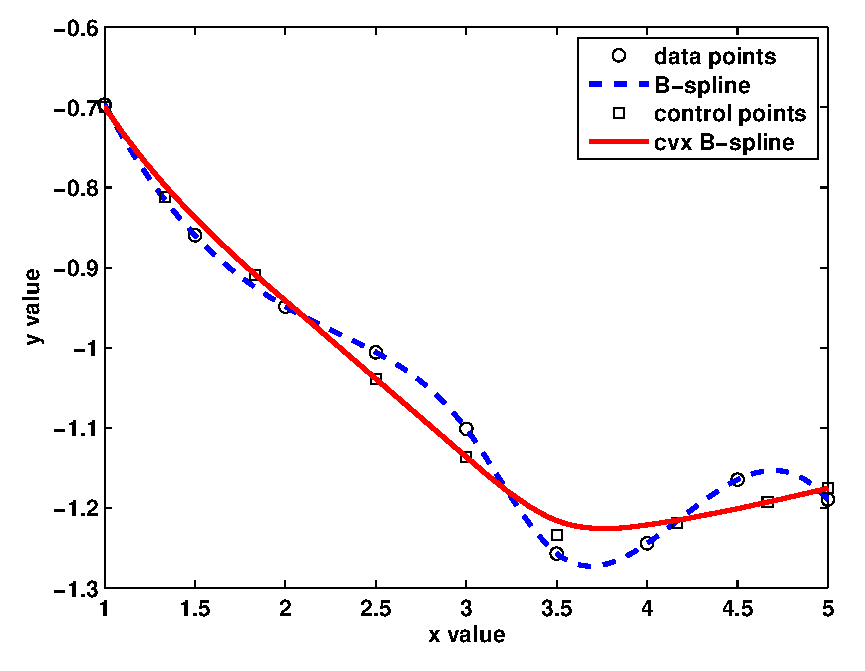
\includegraphics[width=0.45\textwidth]{./figs/cvx1d}
\caption{Univariate convex approximation using B-splines}
\label{fig:1d}}
\end{figure}

\section{Multivariate Approximation by Tensor-Product B-Splines}
\label{sec:2d}
For multivariate cases, the tensor-product B-spline is employed. The
convexity conditions however are not trivial extensions of the
univariate cases. More discussions can be found in~\cite{Floater_99}. 
Without loss of generality, we mainly present the bivariate cases in
this section followed the works by Floater~\cite{Floater_93}.

Given knot sequences $\{u_0\leq\cdots\leq u_{L_1+2m-2}\}$,
$\{v_0\leq\cdots\leq v_{L_2+2n-2}\}$ and the control points
$p_{i,j}\in\setR$ for $i=0,\ldots,L_1+m-1$, $j=0,\ldots,L_2+n-1$.
The \emph{tensor-product B-spline surface} is defined by
\begin{equation}\label{eqn:tp}
S(x,y)=\sum_{i=0}^{L_1+m-1}{
\sum_{j=1}^{L_2+n-1}{B_{i,m}(x)B_{j,n}(y)p_{i,j}}}
\end{equation}
for $u_{m-1}\leq x\leq u_{L_1+m-1}$, $v_{n-1}\leq y\leq v_{L_2+n-1}$,
where $B_{i,m}(x)$ is the $i$th basis function of order $m+1$ over the
$u$ knot sequence and $B_{j,n}(y)$ is the $j$th basis function of
order $n+1$ over the $v$ knot sequence. 

The derivatives of B-splines can be expressed as B-splines
themselves, thus the second derivatives of $S(x,y)$ can be expressed
in the following:
\begin{eqnarray}
S_{xx}(x,y)&=&\sum_{i=2}^{L_1+m-1}{
          \sum_{j=0}^{L_2+n-1}{B_{i,m-2}(x)B_{j,n}(y) a_{i,j}}}
\nonumber\\
S_{xy}(x,y)&=&\sum_{i=1}^{L_1+m-1}{
          \sum_{j=1}^{L_2+n-1}{B_{i,m-1}(x)B_{j,n-1}(y) b_{i,j}}}
\nonumber\\
S_{yy}(x,y)&=&\sum_{i=0}^{L_1+m-1}{
          \sum_{j=2}^{L_2+n-1}{B_{i,m}(x)B_{j,n-2}(y) c_{i,j}}}
\nonumber
\end{eqnarray}
where 
\begin{eqnarray}
a_{i,j}&=&\frac{m(m-1)}{u_{m+i-2}-u_{i-1}}
      \left(\frac{p_{i,j}-p_{i-1,j}}{u_{i+m-1}-u_{i-1}}
           -\frac{p_{i-1,j}-p_{i-2,j}}{u_{i+m-2}-u_{i-2}}\right)\nonumber\\
b_{i,j}&=&mn\frac{p_{i,j}-p_{i-1,j}-p_{i,j-1}+p_{i-1,j-1}}
                {(u_{i+m-1}-u_{i-1})(v_{j+n-1}-v_{j-1})}\nonumber\\
c_{i,j}&=&\frac{n(n-1)}{v_{n+j-2}-v_{j-1}}
      \left(\frac{p_{i,j}-p_{i,j-1}}{v_{j+n-1}-v_{j-1}}
           -\frac{p_{i,j-1}-p_{i,j-2}}{v_{j+n-2}-v_{j-2}}\right).\nonumber
\end{eqnarray}


A twice differentiable function $f:\setR^n\to\setR$ is convex if and
only if for all $\vectorx\in \mathbf{dom}f$ its \emph{Hessian matrix}, 
defined as 
\[H=\left(\frac{\partial^2 f(x)}{\partial x_i \partial x_j}\right),
\quad i,j=1,\ldots,n,\]
is positive semidefinite. 
In bivariate case, this is expressed as  
\[H=\left(\begin{array}{cc}
S_{xx} & S_{xy} \\ S_{yx} & S_{yy}
\end{array}\right) \succeq 0.\]

The Hessian matrix $H_{i,j}$ at control point site
$(u_i^*,v_j^*)$ is calculated from~\cite{Floater_93}.

It has been proved in~\cite{Floater_93} that the Hessian matrices of a
B-spline tensor-product surface are semidefinite if the following
conditions are satisfied and hence the surface is convex.
\begin{thm}[Convex condition of B-spline surface~\cite{Floater_93}]
\label{thm:weak}
Let $S$ be the B-spline surface~(\ref{eqn:tp}) and suppose that $m\geq
2$ and $n\geq 2$. If
\[a_{i,j}\geq 0,\quad \mbox{for }i=2,\ldots,L_1+m-1,
                                ~j=0,\ldots,L_2+n-1,\]
\[c_{i,j}\geq 0,\quad \mbox{for }i=0,\ldots,L_1+m-1,
                                ~j=2,\ldots,L_2+n-1,\]
and
\[\left(\begin{array}{cc}
a_{i,j-l-s} & b_{i-k,j-l} \\ b_{i-k,j-l} & c_{i-k-r,j}
\end{array}\right) \succeq 0.\]
for $i=2,\ldots,L_1+m-1$, $j=2,\ldots,L_2+n-1$, $k,l,r,s\in\{0,1\}$,
then $S$ is convex.
\end{thm}

%% By enforcing $H_{i,j}$ at every control point site to be
%% semidefinite, the whole polygon arc of control points becomes convex,
%% and thus the tensor-product approximation made by these points is
%% convex. 
The approximation problem is formulated as a semidefinite programming:
\begin{equation}\label{eqn:2d_cvx_prog}\begin{array}{ll}
\mbox{minimize} & ||\matrixB \cdot \vectorp - \vectory||_2 \\
\mbox{subject to}& \mbox{the conditions in Theorem~\ref{thm:weak}}
\end{array}
\end{equation}
and can be solved efficiently. Fig.~\ref{fig:2d} gives an example to
illustrate the method. The original data points are taken by sampling of
the Franke's function and is presented in Fig.~\ref{fig:2d_a}. A plot
of the tensor product B-spline generated by MATLAB's Spline Toolbox is
shown in Fig.~\ref{fig:2d_b}. With convexity constraints, the convex
({\it concave} more precisely) B-spline surface is shown in
Fig.~\ref{fig:2d_c}. The corresponding contour plot is shown in
Fig~\ref{fig:2d_d}.

\begin{figure}[!htb]
\subfigure[Original data points.]{
   \label{fig:2d_a}
   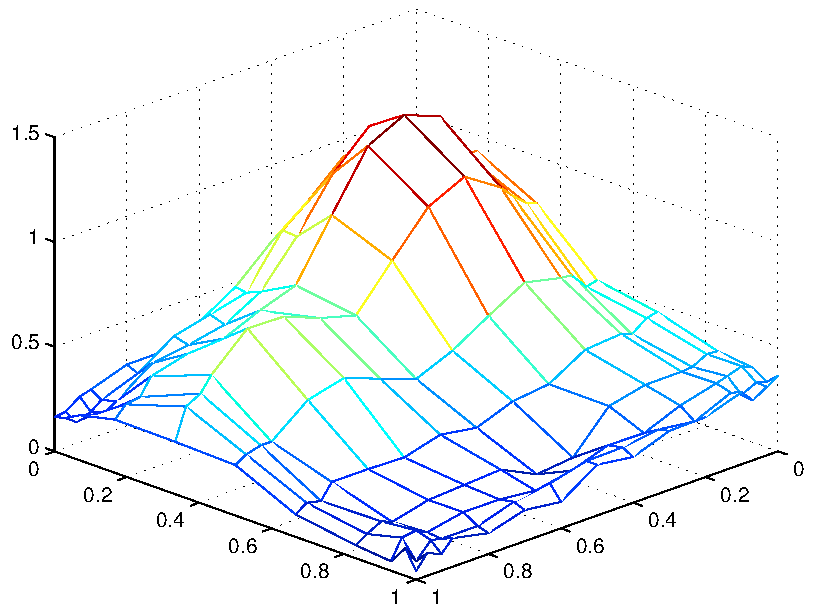
\includegraphics[width=0.23\textwidth]{./figs/cvx2d_data}
}
\subfigure[Least squares B-spline approximation.]{
   \label{fig:2d_b}
   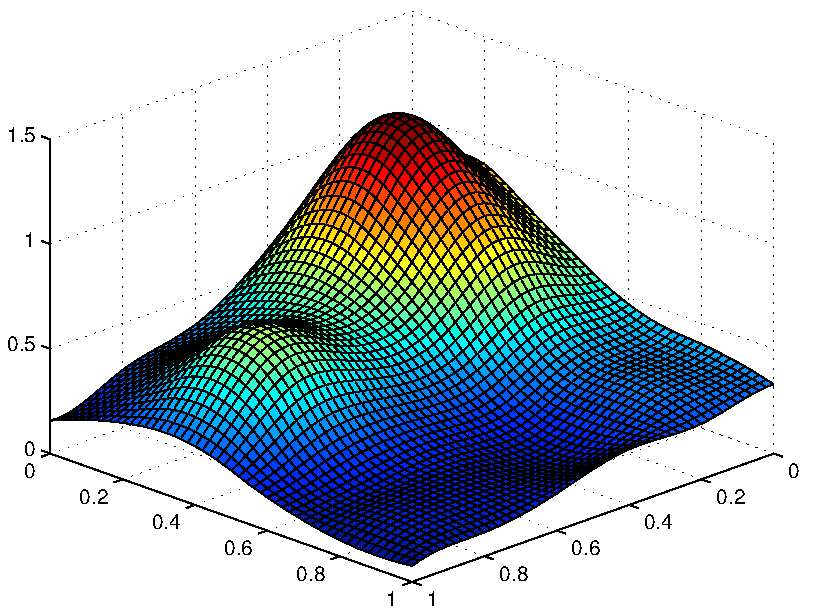
\includegraphics[width=0.23\textwidth]{./figs/cvx2d_spap}
}
\subfigure[Convex tensor-product surface.]{
   \label{fig:2d_c}
   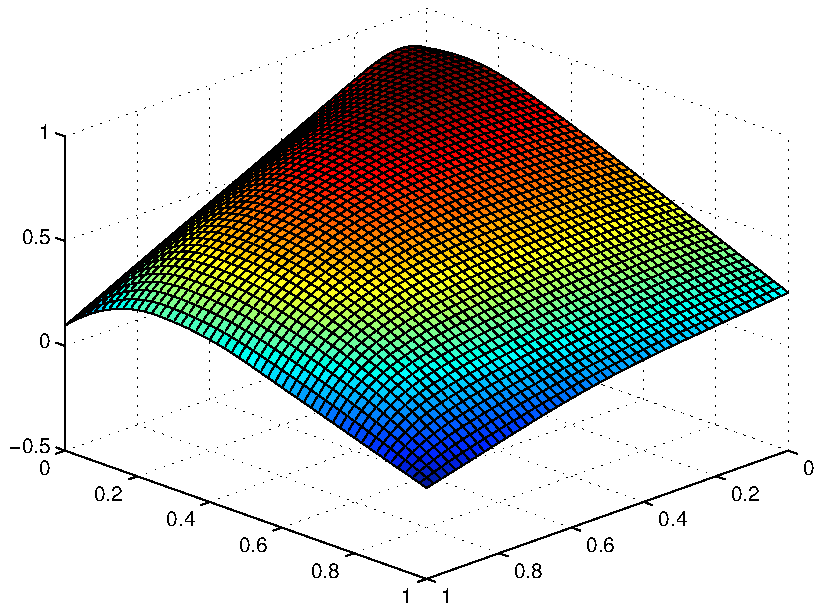
\includegraphics[width=0.23\textwidth]{./figs/cvx2d_cvx}
}
\subfigure[Gradients of convex approximation.]{
   \label{fig:2d_d}
   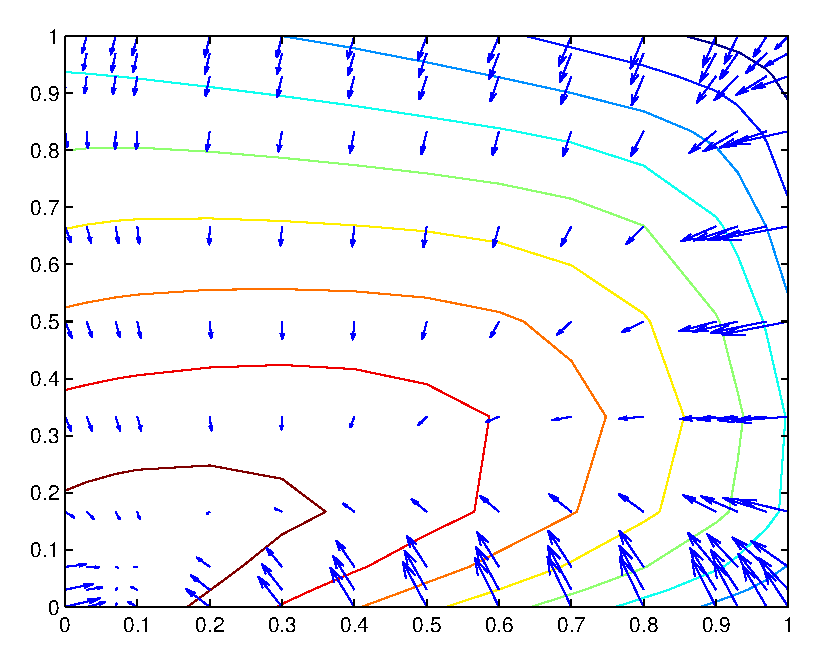
\includegraphics[width=0.23\textwidth]{./figs/cvx2d_dir}
}
\caption{Bivariate convex approximation using tensor-product
  B-splines.} 
\label{fig:2d}
\end{figure}

\section{Experimental Results}\label{sec:example}
In this section, we will describe two simple circuit examples and show
the performance of our approach. A publicly available MATLAB based
package, the CVX~\cite{cvx_pack}, is applied for our convex B-spline
approximation. CVX is a system for disciplined convex
programming (DCP), and has the proficiency in solving semidefinite
programming and the convex optimization in our case. 
All the designs are simulated and verified in a CMOS 0.18$\mu$m
process, and the simulator is HSPICE.

\subsection{Buffer modeling example}
In VLSI design, the standard cells are frequently used circuit modules
and their performances in special circumstances require fine
tuning. Here we take a CMOS buffer for an instance, whose
gate delay is our primary interest. In this model, gate
delay depends on three parameters: input slew, drive strength, and
load capacitance. Previously, a posynomial fitting method is applied
to find the delay model of a CMOS invertor in~\cite{Roy_05}, in which
three different algorithms to solve this fitting problems are
developed. This is because finding a universally accurate posynomials
for every circuit case is exceptionally difficult. The algorithms
in~\cite{Roy_05}
make the invertor model convexified and smoothed. However, their point
addition method could not always guarantee convexity.

Our algorithm is capable of modeling this kind of standard cells, and
smoothness and convexity are both ensured. The buffer we used as an
example has two serial invertors inside, 
therefore the slew of input signal, load capacitance and the size of
the four transistors will have a combined effect on the gate delay. In
Fig.~\ref{fig:bf_o_sl} the delay versus input slew 
and load is illustrated, and the convex approximation by our approach 
is plotted in Fig.~\ref{fig:bf_o_sc}. The comparison
between original data surface and the modeling surface of our
method prove that smoothness and convexity are both preserved. 

\begin{figure}[!tb]
\subfigure[Original data of gate delay vs. slew and load.]{
   \label{fig:bf_o_sl}
   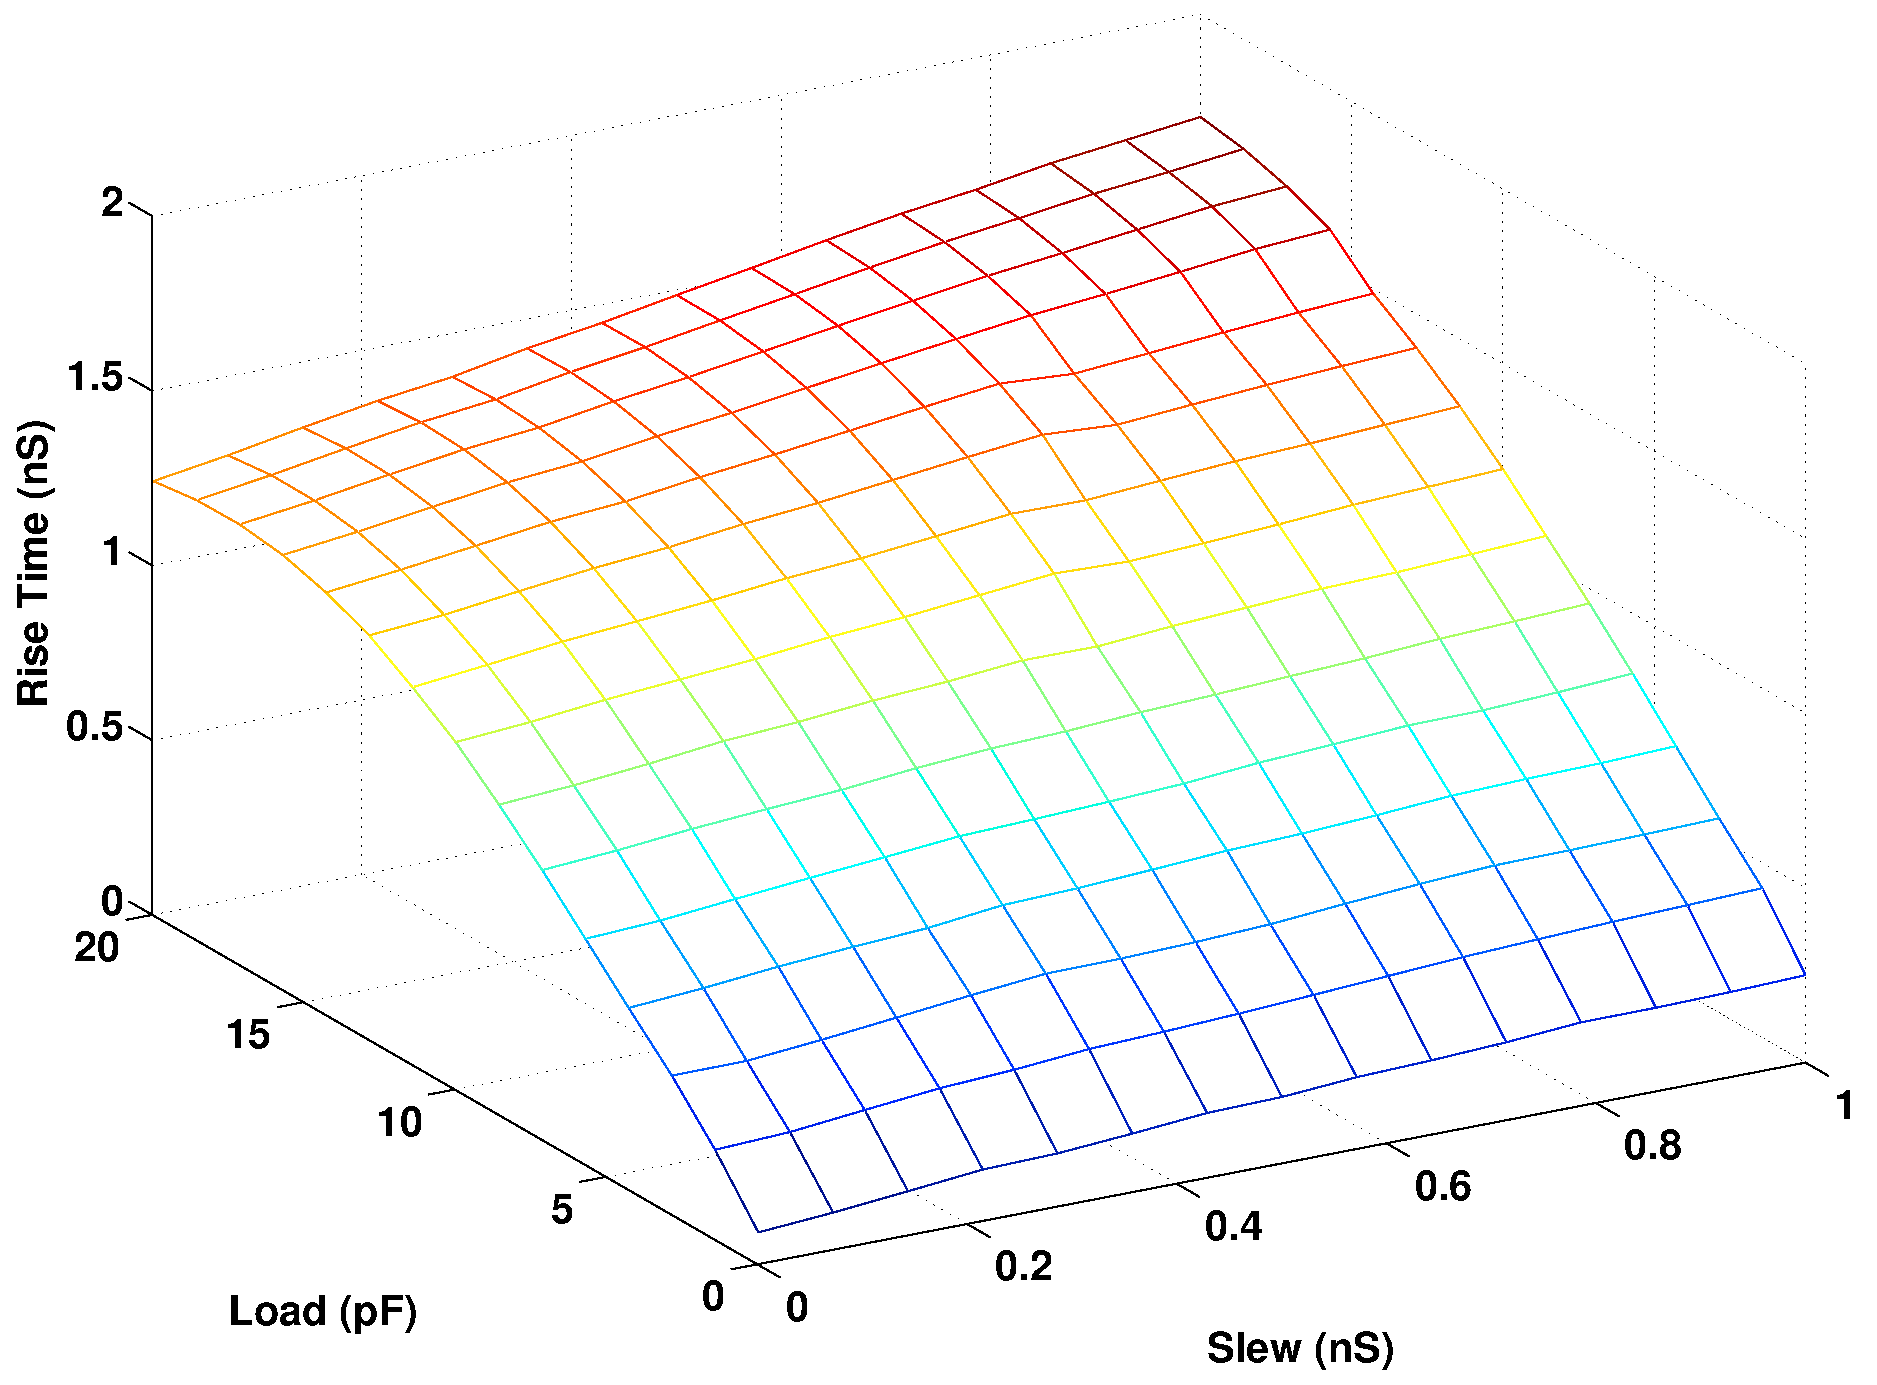
\includegraphics[width=0.23\textwidth]{./figs/buffer_RD_slew_load}
}
\subfigure[Convex approximation of gate delay vs. slew and load.]{
   \label{fig:bf_o_sc}
   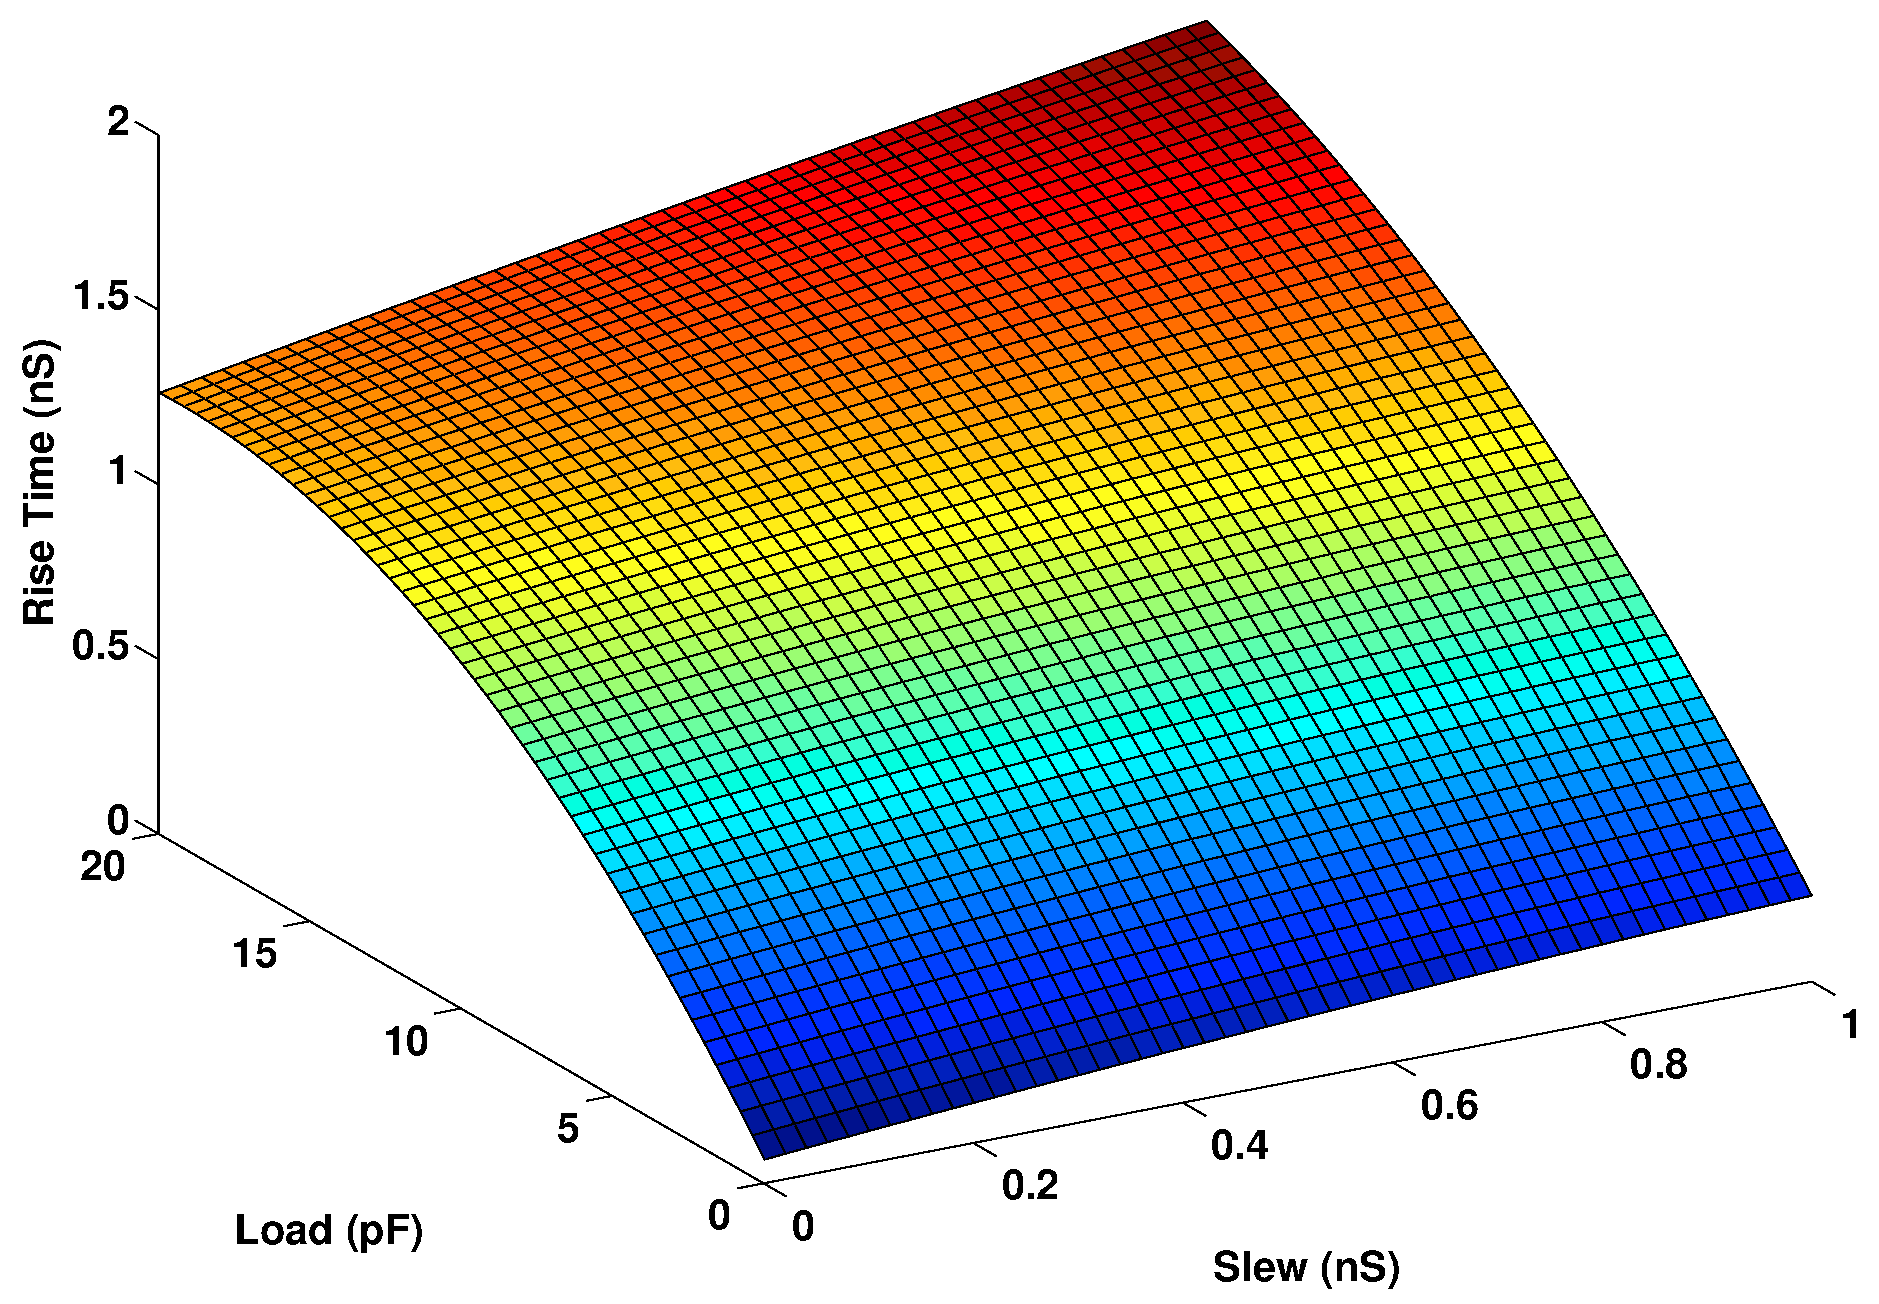
\includegraphics[width=0.23\textwidth]{./figs/cvx_buffer}
}
\caption{Modeling of a buffer by proposed method.} 
\label{fig:buffer}
\end{figure}


\subsection{Op Amp optimization example}
To demonstrate the practicability, a two-stage CMOS op-amp in
Fig.~\ref{fig:opamp} is used for modeling and sizing. After the basic
analysis of this circuit, it is possible to formulate most
specification and performance functions in convex
forms via geometric programming~\cite{GP_OpAmp}. In such scenarios,
using a completely precise 
model of the circuit at several beginning iterations is
unnecessary. To save much simulation time as well as guarantee the
accuracy in the end, a coarse to refined approximation is a good
choice. The starting point of our simulation is found by a random
chosen one which satisfies the circuit's working condition, and around
this point a sparse data grid is constructed and sampled. The
performance data obtained from the simulations on the grid then serve
to approximate a model. As the iterations repeat, the data grid
becomes dense and the scope of sampling retracts compared to the
former one. 

The specifications for the circuit design
and the performances of the circuit after the sizing iterations are
listed in Table~\ref{tab:spec}, where we have the Unity-Gain Frequency
maximized while other constraints are not violated. It is shown that
even though the starting design does not meet the specifications, our
final result suffices to go along with them.

\begin{figure}[!tb]{\centering
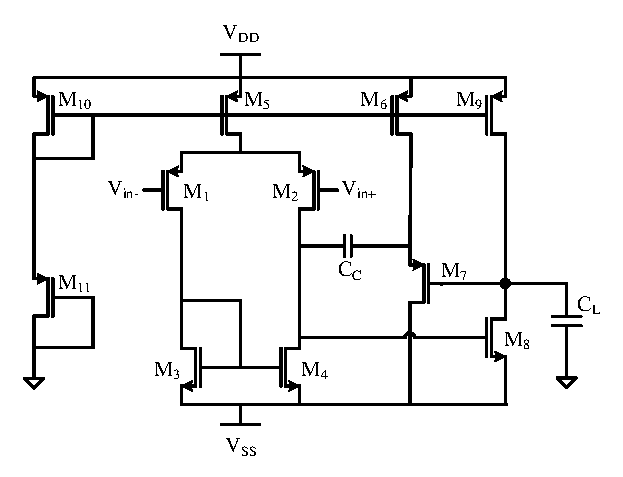
\includegraphics[width=0.4\textwidth]{./figs/two-stage}
\caption{Two-stage CMOS Op-Amp.}
\label{fig:opamp}}
\end{figure}

\begin{table}[!htb]
  \centering
  \caption{Performance of Op-Amp under sizing procedure.}\label{tab:spec}
  \begin{tabular}{|c|c|r|r|}
    \hline
               &\multicolumn{1}{|c|}{Spec}&\multicolumn{1}{|c|}{Initial}&\multicolumn{1}{|c|}{Final}\\
    \hline\hline
    Gain (dB)              &$\geq 60$& 82 & 64    \\
    Unity Gain Freq. (MHz) &  max    & 1.85 & 9.44  \\
    Phase Margin (degree)  &$\geq 60$& 47 & 65    \\
    Slew Rate (V/$\mu$s)   &$\geq 20$& 31 & 23    \\
    Power (mW)             &$\leq 5$ & 5.4 & 3.7   \\ 
    \hline
  \end{tabular}
\end{table}


\section{Conclusions}\label{sec:conclusion}
In this paper we have presented an new approach to approximate the
characteristic functions of analog circuits by tensor-product B-splines. These
approximated functions relate the performance and specification to the
design parameters, therefore can be used in further applications such as
circuit sizing. In favor of the convex nature of some circuits, the
proposed method has the ability to retain convexity and
thus facilitate the convex optimization of the circuit to efficiently
find the optimal result. We demonstrate this approach with two
examples: gate delay of a buffer is modeled, and a two-stage CMOS
amplifier is optimized to meet prescribed specification and achieve
its largest bandwidth. 

\bibliographystyle{unsrt}
 \scriptsize
\bibliography{ref-cvxfit,refbibtex,ref-fitting}

\end{document}
